
\chapter{Integrity and attestation of distributed infrastructures (cloud, SDN, NFV, …) \textbf{Appunti AI CORREGGERE}}

\section{Introduction}

\subsection{Typical distributed infrastructures}

\begin{figure}[h]
    \centering
    \shadowbox{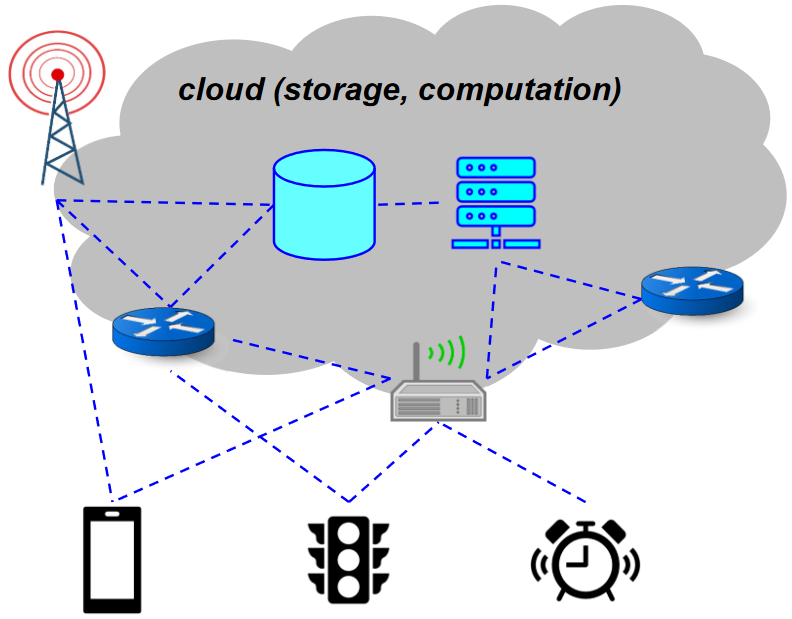
\includegraphics[width=0.4\textwidth]{img/dist-arch.png}}
    \caption{Distributed infrastructure}
    \label{fig:distributed_infrastructure}
\end{figure}


\begin{enumerate}[itemsep=0pt]
    \item Cloud computing (Server, Storage ...)
    \item edge devices (Router, Switch,modems  \dots) for guarantee access the cloud
    \item IoT and personal devices (Smartphone, robot cleaner,  \dots) for use the data and services
\end{enumerate}

All these conncection are different (wired, wireless, virtulized, \dots) and the secure all these kind of connection is very hard.

\subsection{Trend towards softwarization}

So now a lot of hardware device are repliaced by software, this is a trend that is called \textbf{softwarization}.

\begin{itemize}[itemsep=0pt]
    \item \textbf{SDN (Software-Defined Networking)}
    \item \textbf{... but also:}
    \begin{itemize}[itemsep=0pt]
        \item SDR, NFV, ...
        \item AI (!)
    \end{itemize}
    \item \textbf{As a consequence, more flexible but more vulnerable:}
    \begin{itemize}[itemsep=0pt]
        \item Software more prone to bugs than hardware
        \item Software updates (if you receive an update, is it trusted? it include a malware?)
    \end{itemize}
\end{itemize}

\begin{boxH}
- EASY (FAST, FLEXIBLE, ...) \\
- CHEAP \\
- SECURE \\
... PICK TWO!
\end{boxH}

\subsubsection{Can I trust this infrastructure?}
A trustworthy infrastructure is defined as one that will behave in the expected way. However, several \textbf{problems} arise in achieving this trust:

\begin{itemize}[itemsep=0pt]
    \item Trust in the cloud provider(s) (as HW, as SW, as people managing the infrastructure)
    \item Trust in the network/edge provider(s) (as cloud)
    \item Low or no access control for edge- and end-devices
    \item Low-cost IoT devices (typically implying low security, so most of them are completely unsecure) 
    \item Personal devices (typically managed by "ignorant" users)
\end{itemize}

If possible, the infrastructure should be protected to avoid or block attacks. Otherwise, it is essential to \textbf{at least monitor the "state"} of the system for early detection and possible reaction.\\ Some of this work is done with IDS, but can't find all the possible attacks, so we need to do some \textbf{Integrity Verification}

\subsection{Integrity}
\textbf{Hardware:}
\begin{itemize}[itemsep=0pt]
    \item Am I talking to the right (intended) node?
    \item Does it host the expected (physical) components?
\end{itemize}

\textbf{Software:}
\begin{itemize}[itemsep=0pt]
    \item Am I talking to the right (intended) software component?
    \item Is it correctly configured?
    \item Is the baseline software the expected one?
\end{itemize}

\section{TEE - Trusted Execution Environment}

A small part of the system that is isolated from the rest of the system, and that is trusted to execute some code in a secure way.

\subsection{Trusted vs. Trustworthy}

- \textbf{Trusted} refers to someone or something that you rely upon to not compromise your security. On the other hand, \textbf{Trustworthy} refers to someone or something that will not compromise your security. \\
- \textit{Trusted} is about how you use something, while \textit{Trustworthy} is about whether it is inherently safe to use. \\
- A \textbf{Trusted Execution Environment} is what you may choose to rely upon to execute sensitive tasks, such as running \textbf{Trusted Applications (TA)}. This environment should be \textbf{Trustworthy} as well!

\subsection{TEE evolution}
The evolution of the \textbf{Trusted Execution Environment (TEE)} has gone through several significant milestones. \bigskip

\textbf{Open Mobile Terminal Platform (now part of GSMA)} started the initiative.
\begin{itemize}[itemsep=0pt]
    \item \textbf{2006}: Introduction of the \textbf{TR0 specifications}, outlining the basic security requirements.
    \item \textbf{2008}: Release of the \textbf{TR1 specifications}, which added the TEE layer on top of TR0.
    \item \textbf{2010}: \textbf{GlobalPlatform} was launched to define interfaces and provide certifications, becoming the de-facto standardization body for TEEs.
    \item \textbf{2012}:
    \begin{itemize}[itemsep=0pt]
        \item \textbf{ARM}, \textbf{Gemalto}, and \textbf{G+D} formed \textbf{Trustonic}, aiming to create an open TEE.
        \item \textbf{GlobalPlatform} and the \textbf{Trusted Computer Group (TCG)} created a joint working group to focus on TEE specifications and its use combined with the \textbf{Trusted Platform Module (TPM)}.
    \end{itemize}
\end{itemize}
The first major business case for the Trusted Execution Environment (TEE) was Netflix's high-resolution content on smartphones and tablets. Following this, TEE's application rapidly expanded into various sectors, including financial services, enterprise solutions, government security, automotive industries, and the Internet of Things (IoT)

\subsection{TEE and REE}
\begin{figure}[h]
    \centering
    \shadowbox{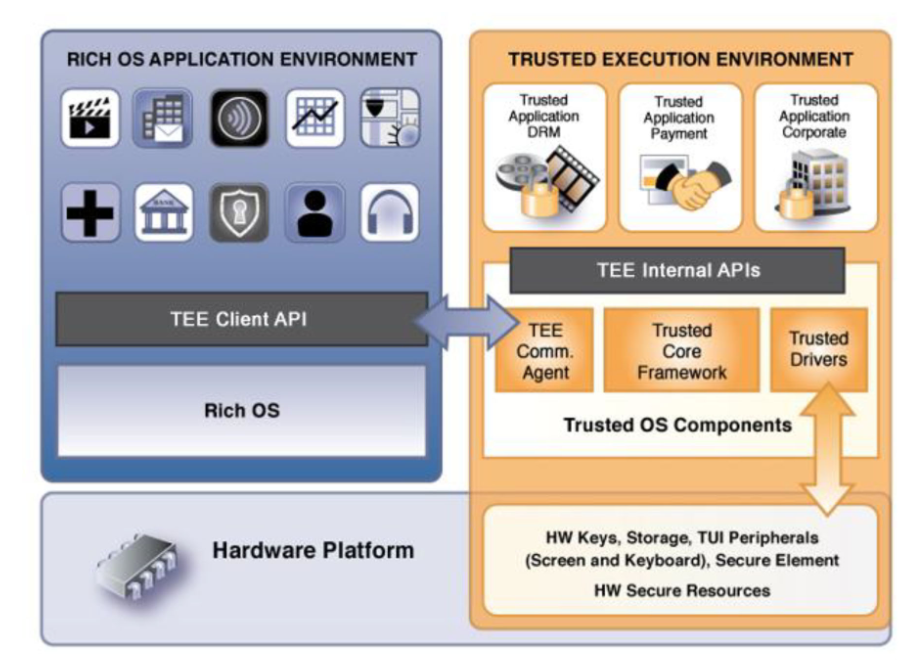
\includegraphics[width=0.4\textwidth]{img/tee-ree.png}}
    \caption{TEE and REE}
    \label{fig:tee_ree}
\end{figure}
(recuperare descrizione da transcript)
\begin{itemize}[itemsep=0pt]
    \item \textit{Note:}
    \item TUI: Trusted User Interface
    \item TEE run only on device that respect RT0 specifications
    \item The most risky part is the communication between TEE client API and TEE internal APIs 
\end{itemize}


\subsection{TEE - Some key points}
\textbf{Trusted Execution Environment (TEE)} is currently a hot topic in the realm of \textit{confidential computing}, which is promoted by the \textbf{Confidential Computing Consortium (CCC)}.\\ One of the key objectives of TEE is the protection of \textbf{data in use}, ensuring that no unauthorized entity can read or write this data, and it is processed only by an authorized application. This is in contrast to various cryptographic techniques used to protect \textit{data at rest} and \textit{data in motion}. \bigskip

A critical component of TEE is the \textbf{Root of Trust (RoT)}, an element whose misbehavior cannot be detected during runtime (it's trusted and stop). It is essential that the RoT be both \textit{trusted} and \textit{trustworthy}. The RoT is part of the \textbf{Trusted Computing Base (TCB)}, which includes all hardware, firmware, and software components that are crucial to the system's security. Any vulnerability within the TCB could potentially jeopardize the security of the entire system.

\subsection{TEE Security Principles}

Trusted Execution Environments (TEEs) are built on foundational security principles to ensure the confidentiality and integrity of sensitive tasks. These principles include:

\begin{itemize}
    \item Being part of the device's secure boot chain, which is based on a Root of Trust (RoT). This ensures code integrity is verified during each device boot.
    \item Hardware-based isolation from the rich operating system (OS) environment, allowing sensitive code execution in a protected manner.
    \item Isolation of Trusted Applications (TAs) from each other to prevent interference or data leakage.
    \item Secure data storage, leveraging a hardware-unique key accessible only by the TEE OS. This prevents unauthorized access, modification, or exploitation of data across devices.
    \item Privileged and secure access to peripherals (also known as a trusted path). For instance, peripherals like fingerprint sensors, displays, and touchpads can be isolated from the rich OS environment and controlled solely by the TEE during specific operations. This setup ensures no visibility or access from the Rich Execution Environment (REE), including from potential malware.
\end{itemize}


\subsection{Intel IPT}

\textbf{Intel Identity Protection Technology (IPT)} is a security feature that runs a Java applet on a separate CPU. The \textbf{Management Engine} is part of the chipset, meaning it is bound to the physical hardware. This setup enables a variety of secure applications, including:

\begin{itemize}
    \item Key generation and storage (integrated with Windows Cryptographic API)
    \item One-Time Password (OTP) generation (e.g., VASCO MYDIGIPASS.COM)
    \item Secure PIN entry
    \item \begin{itemize}
        \item These features are made possible because the chipset also manages video
    \end{itemize}
\end{itemize}

\subsection{ARM TrustZone}

\textbf{ARM TrustZone} extends CPU buses to a "33rd bit," which signals whether the CPU is in secure mode or not. This signal is exposed outside of the CPU, enabling the use of secure peripherals and secure RAM. 

Key characteristics include:
\begin{itemize}
    \item The system is open and well-documented.
    \item \textbf{But}, it only allows for \textit{one} secure enclave.
    \item ARM is working on adding a \textit{third mode} to enhance its capabilities.
\end{itemize}

Additionally, there is potential for an indicator to signal the current mode the CPU is operating in.

\subsection{Trustonic}

TrustZone by itself is limited due to only allowing one secure enclave, but several companies have developed solutions to overcome this limitation:
\begin{itemize}
    \item \textbf{Gemalto} developed the \textit{Trusted Foundations system}.
    \item \textbf{G+D (Giesecke+Devrient)} developed \textit{MobiCore}.
    \item Both of these solutions essentially split the one secure enclave into several ones, using a smart-card-like operating system.
\end{itemize}

\textbf{Trustonic's} development is based on MobiCore, and license fees are required to implement its code. 

Trustonic’s TEE OS, \textbf{Kinibi}, powers various systems, such as version 500, which supports 64-bit SMP for embedded systems.

\textbf{Samsung Knox} provides a similar functionality, but also introduces secure boot for added security.


\subsection{Intel SGX}

Intel Software Guard Extensions (SGX) is a security feature tightly integrated with the CPU, designed to modify memory management and enhance protection for enclaves. These enclaves are isolated from other code, ensuring that their contents are secure and cannot be accessed by unauthorized code.

Key features include:
\begin{itemize}
    \item As enclaves are built, the code is measured in a manner similar to TPM, ensuring integrity.
    \item SGX can be combined with Intel Identity Protection Technology (IPT) for trusted display functionality.
    \item Initially, \textbf{SGX1} was available on both low- and high-end CPUs, but now \textbf{SGX2} is mostly restricted to server-oriented CPUs, such as Xeon processors.
\end{itemize}


\subsection{Keystone}

Keystone is an open-source framework designed to build Trusted Execution Environments (TEEs) with flexibility and modularity. The key features include:

\begin{itemize}
    \item An open-source framework that allows developers to select only the required features, reducing the Trusted Computing Base (TCB) to a minimum.
    \item It operates in an untrusted environment, typically a general-purpose OS, while supporting multiple trusted and segregated enclaves.
\end{itemize}
\begin{itemize}
    \item Built on top of the RISC-V open-source customizable hardware architecture.
    \item Can be implemented on FPGA or SoC platforms, with a core that includes cryptographic extensions.
    \item Supports various execution modes: Machine (M), Supervisor (S), and User (U).
    \item Physical Memory Protection (PMP) is utilized for both memory and I/O protection, ensuring secure execution and isolation (So create a secure page that can give to a process and this page is not accessible from the other process).
\end{itemize}

\subsubsection{Motivation for Keystone}

The motivation behind Keystone arises from the limitations of existing Trusted Execution Environments (TEEs), which are often rigid and lack customizability. Several existing solutions inherit significant design constraints, such as:

\begin{itemize}
    \item \textbf{Intel SGX}: Characterized by a large software stack, which introduces complexity and a lot of libaries (so a big trust in Intel).
    \item \textbf{AMD SEV}: Involves a large Trusted Computing Base (TCB), need a large use of software, so a large trusted domanin
    \item \textbf{ARM TrustZone}: Restricts flexibility due to the limited number of secure domains it can handle.
\end{itemize}

Keystone aims to address these issues by providing a more customizable, modular TEE framework.

\subsubsection{Keystone architecture}
\begin{figure}[h]
    \centering
    \shadowbox{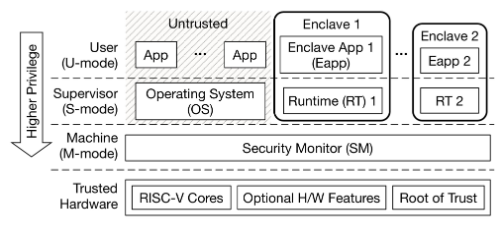
\includegraphics[width=0.4\textwidth]{img/keystone-arch.png}}
    \caption{Keystone architecture}
    \label{fig:keystone_architecture}
\end{figure}

\begin{itemize}
    \item risc-v core: normal operations
    \item Root of trust: needed
    \item Optional H/W features: can be added
    \item Security Monitor: The only program that run in Machine mode, and mediates all the operations that are sent to the HW.
    \item At User level, we can have all the untrusted applications.
    \item between U and S mode, we can create all the enclaves that we want (Enclave app (Eapp) at U-mode and Enclave runtime (RT) at S-mode)
\end{itemize}

\subsubsection{Keystone: Further Reading}

\begin{boxH}
    \textbf{Documenti da leggere per l'esam}e
\end{boxH}

For those interested in exploring Keystone in more detail, here are some useful resources:

\begin{itemize}
    \item \textbf{Keystone presentation at CCC}:
    \begin{itemize}
        \item Video: \href{https://www.youtube.com/watch?v=ITA3FfjKqNk}{youtube}
        \item Slides: \textit{CCCWebinar-Keystone.pdf} (available in course material)
    \end{itemize}
    
    \item \textbf{Keystone presentation at EuroSys'20}:
    \begin{itemize}
        \item Slides: \textit{233\_lee\_slides.pdf} (available in course material)
        \item Video: \href{https://www.youtube.com/watch?v=S8MmKBCoPSg}{youtube}
        \item Paper: \href{https://n.ethz.ch/~sshivaji/publications/keystone_eurosys20.pdf}{n.ethz.ch} (also available in course material)
    \end{itemize}
\end{itemize}

\section{Trusted computing and remote attestation}

\subsection{Baseline Computer System Protection}

Attackers often aim to inject malware at the lowest possible level to stay undetected and gain control over large portions of a system. Common tactics include:

\begin{itemize}
    \item Modifying the operating system (OS)
    \item Attempting to boot an alternative OS
    \item Altering the boot sequence or boot loader (for start an untrusted part)
\end{itemize}

To counter these threats, it is essential to protect the boot system and the OS itself. In earlier systems, the BIOS was used, but it was very difficult to secure (no support to signature). Now, with the advent of UEFI, systems have:

\begin{itemize}
    \item Native support for firmware signature and verification
    \item The ability for the boot loader to verify the OS before activation
\end{itemize}

\subsection{Rootkits}

Rootkits are malicious software designed to gain privileged access by infiltrating different layers of a computer system. Common types include:

\begin{itemize}
    \item \textbf{Firmware rootkits:} These overwrite the BIOS/UEFI or the firmware of other hardware components (like a network card for a server, that have another processor and firmware, so it can be object of an attack), allowing the rootkit to start before the operating system (OS) loads.
    
    \item \textbf{Bootkits:} These replace the OS's bootloader, enabling the system to load the bootkit before the OS, compromising the system early in the boot process.
    
    \item \textbf{Kernel rootkits:} These modify portions of the OS kernel, ensuring the rootkit loads automatically when the OS starts, giving the attacker control at the core level.
    
    \item \textbf{Driver rootkits:} These impersonate trusted hardware drivers, such as those used by operating systems like Windows, to communicate with hardware, allowing the rootkit to operate undetected.
\end{itemize}


\begin{boxH}
\textbf{Software to Protect Software?} \bigskip

Relying solely on software to protect other software is generally \textit{not} a good idea, as software can fail. To ensure robust protection, hardware support is necessary for safeguarding software. A key element in this context is the \textbf{Root of Trust (RoT)}, which should be part of the \textbf{Trusted Computing Base (TCB)}. This is essential because hardware itself is operated by software or firmware. Therefore, the TCB should be kept minimal to reduce potential vulnerabilities.

\end{boxH}


\subsection{Firmware Self-Protection (SW Root-of-Trust)}

\textbf{Example courtesy of HPE.}
\begin{enumerate}[itemsep=0pt]
    \item HPE has a \textit{signature} region at a fixed location in the final BIOS image (16MB).
    \item After the BIOS build (i.e., at manufacturing time), the SHA256 of specific BIOS regions is calculated; these regions include static code, the BIOS version information, and microcode.
    \item The hash is sent to the HPE signing server, which returns a signed hash image (32 bytes + signature and certificate size), which is copied into the \textit{signature} region.
    \item After power-on, the early BIOS code calculates the combined hash of each of the specific valid regions in the BIOS image.
    \item After verifying that the \textit{signature} region contents are valid, the BIOS compares the stored hash and the calculated hash.
    \item If both are the same, the boot continues; otherwise, the system halts.
\end{enumerate}


\subsubsection{HW root-of-trust for firmware protection}
For hardware root-of-trust, self-verification is based on the firmware itself, where the static portion verifies the updatable part. However, an external chip can also be used to verify the firmware, as shown in the system diagram below. The external crypto chip validates the BIOS in the SPI flash after power-on. Only once validation is successful does the x86 CPU exit reset mode; otherwise, the system remains in a reset state.

\begin{wrapfigure}{r}{0.4\textwidth}
    \centering
    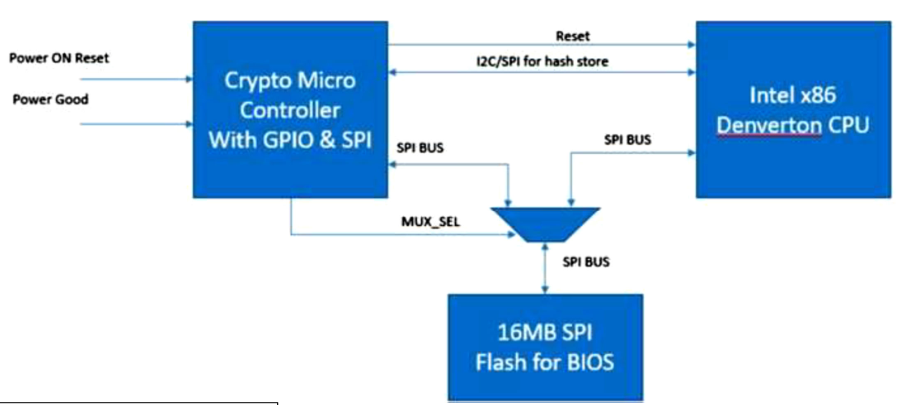
\includegraphics[width=0.4\textwidth]{img/hw-rot-for-firmware.png}
    \caption{Firmware Root of Trust - System Diagram}
\end{wrapfigure}

This chip also includes a fusing option, enabling one public key hash to be fused, which will be used to verify the signature of the hash file stored in the "signature" region. The validation flow is similar to the BIOS self-integrity check, but with the external chip performing the validation, it establishes the real hardware root of trust.

\subsection{Boot Types}

There are several types of boot processes with varying degrees of security. 


\begin{itemize}[itemsep=0pt]
    \item The simplest type is the \textbf{plain boot}, which offers no security mechanisms at all, making the system vulnerable to attacks.
    \item \textbf{Secure boot} ensures that the firmware verifies the signature of critical components and will halt the platform if the verification fails. This type of boot is mostly hardware-based, verifying components up to the OS loader.
    \item \textbf{Trusted boot} goes further by having the OS verify the signature of its components, such as drivers and antimalware. If the verification fails, the OS will stop operations. Trusted boot is primarily software-based and ensures verification up to the OS operational state.
    \item \textbf{Measured boot} records measurements of all components executed from the beginning of the boot process up to a defined point (X). Unlike secure and trusted boot, it does not stop operations when an issue is detected but can securely report these measures to an external verifier for further analysis.
\end{itemize}

\begin{figure}{ht}
    \centering
    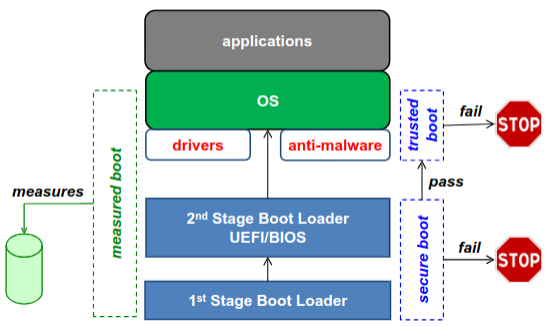
\includegraphics[width=0.4\textwidth]{img/boots.png}
    \caption{Hardware Root of Trust - System Diagram}
\end{figure}

\textit{Note:} trusted driver and antimalware start before the OS

\begin{wrapfigure}{r}{0.4\textwidth}
    \centering
    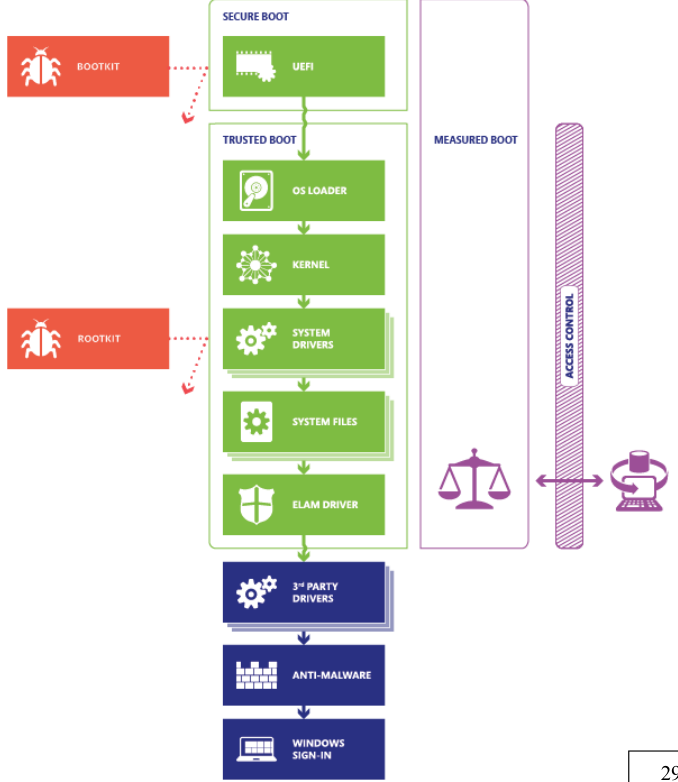
\includegraphics[width=0.4\textwidth]{img/windowd-boot.png}
    \caption{Windows boot protection}
\end{wrapfigure}

\textit{Note:} ELAM: Early Launch Anti-Malware (signed by Microsoft)

\subsection{Trusted Computing}

Trusted Computing refers to schemes that establish trust in a platform by identifying its hardware and software components. A trusted component or platform is one that behaves as expected, though it is important to note that trust is not synonymous with being good or secure. For trust to be meaningful, the component's behavior must be verified against its expected behavior.

One key element in Trusted Computing is \textit{attestation}, which provides verifiable evidence of the platform’s state. The \textit{Root of Trust} (RoT) represents an inherently trusted component in this context, forming the foundation upon which trust is established.

A central part of Trusted Computing is the \textit{Trusted Platform Module} (TPM). The TPM is responsible for collecting and reporting the identities of a platform's hardware and software. In a typical system, the TPM reports on these components in a way that allows the system to determine whether their behavior aligns with expectations, thereby establishing a trusted environment.


\subsection{Trusted Computing Base (TCB)}

The \textit{Trusted Computing Base (TCB)} is the collection of system resources, including both hardware and software, responsible for maintaining the system's security policy. One critical attribute of the TCB is its ability to protect itself from being compromised by any hardware or software that is not part of the TCB.

It is important to note that the \textit{Trusted Platform Module (TPM)} is not the TCB of a system. Instead, the TPM serves as a component that enables an independent entity to determine if the TCB has been compromised. In certain situations, the TPM can assist in preventing the system from starting if the TCB cannot be properly instantiated.

\subsection{Root of Trust (RoT)}

The \textit{Root of Trust (RoT)} refers to a component that must always behave as expected, as its misbehavior cannot be detected. It forms the fundamental building blocks for establishing trust in a platform. There are three main types of RoT:

\textbf{Root of Trust for Measurement (RTM)}:  
Responsible for measuring system integrity and sending integrity measurements to the \textbf{RTS}. Typically, the CPU runs the \textit{Core Root of Trust for Measurement (CRTM)} at boot, as the first piece of BIOS/UEFI code, initiating the chain of trust (because we want that all that is executed is mesure).

\textbf{Root of Trust for Storage (RTS)}:  
Provides shielded and secure storage for sensitive information

\textbf{Root of Trust for Reporting (RTR)}:  
Securely reports the content of the RTS, ensuring reliable communication of the platform’s integrity status.


\subsection{Chain of Trust}

The \textit{Chain of Trust} is a sequential process where each component measures the integrity of the next component in the system. The process proceeds as follows:

\textbf{Component A} (typically the \textit{Core Root of Trust for Measurement}, CRTM) measures the integrity of \textbf{Component B} and stores the measurement in the \textit{Root of Trust for Storage (RTS)}. Next, \textbf{Component B} measures \textbf{Component C} and similarly stores the measurement in the RTS. This process continues for each subsequent component.

An important point to note is that a verifier, by using the \textit{Root of Trust for Reporting (RTR)}, can securely retrieve the measurements of components like B and C from the RTS. However, components B and C can only be trusted if \textbf{Component A} (the CRTM) is trustworthy, ensuring the integrity of the entire system chain.


\section{Trusted Platform Module (TPM) overview}

The Trusted Platform Module (TPM) is an \textbf{inexpensive component}, typically costing less than \$1, and is available on most servers, laptops, and PCs. It is designed to be \textbf{tamper-resistant}, although it is important to note that it is not tamper-proof.

While the TPM is\textbf{ not a high-speed cryptographic engine} and is generally considered rather slow, it is certified with a \textbf{Common Criteria EAL4+ rating}. The TPM acts as a \textbf{passive component that requires a CPU} to function effectively.

Although the TPM cannot prevent the boot process, it can protect data and securely report it. In this context, the TPM serves as both an RTS (Root of Trust for Storage) and an RTR (Root of Trust for Reporting), but it is not classified as an RTM (Root of Trust for Measurement).

\subsection{TPM Features}

The Trusted Platform Module (TPM) provides several important features:

\begin{itemize}[left=0pt]
    \item \textbf{RTS}: Secure storage (extend-only).
    \item \textbf{RTR}: Reports the content of the RTS with a digital signature.
    \item Hardware random number generator.
    \item Supports various cryptographic algorithms, including hash, MAC, symmetric, and asymmetric encryption. \\ However, it is \textbf{NOT a crypto accelerator} and is considered slow.
    \item Secure generation of cryptographic keys for limited uses.
    \item \textbf{Binding}: Data encrypted using the TPM bind key, a unique RSA key descending from a storage key.
    \item \textbf{Sealing}: Similar to binding, but specifies the TPM state required for the data to be decrypted (i.e., unsealed).
    \item Computer programs can use a TPM to authenticate hardware devices, as each TPM chip has a unique and secret \textbf{Endorsement Key} (EK) burned in during production.
\end{itemize}

\subsection{TPM-1.2}
The Trusted Platform Module (TPM) version 1.2 includes a fixed set of algorithms, specifically SHA-1, RSA, and optionally AES. It features one storage hierarchy for the platform user and provides a single root key known as the \textbf{Storage Root Key (SRK)}, which uses RSA-2048 encryption. The TPM establishes hardware identity through the built-in \textbf{Endorsement Key (EK)} and supports sealing to \textbf{Platform Configuration Register (PCR)} values.

\subsection{TPM-2.0}
The Trusted Platform Module (TPM) version 2.0 offers enhanced features, including cryptographic agility with support for algorithms such as SHA-1, SHA-256, RSA, ECC-256, HMAC, and AES-128. It introduces three key hierarchies: \textbf{platform}, \textbf{storage}, and \textbf{endorsement}, allowing for multiple keys and algorithms within each hierarchy. Additionally, TPM 2.0 implements policy-based authorization, enabling more flexible security management. Furthermore, it provides platform-specific specifications for various environments, including:
\begin{itemize}
    \item \textbf{PC client}, 
    \item \textbf{mobile} 
    \item \textbf{automotive-thin}
\end{itemize}


\subsubsection{Implementation of TPM-2.0}

The Trusted Platform Module (TPM) 2.0 can be implemented in various ways:

\begin{itemize}[left=0pt]
    \item \textbf{Discrete TPM}: A dedicated chip that implements TPM functionality in its own tamper-resistant semiconductor package.
    \item \textbf{Integrated TPM}: A part of another chip that is not required to implement tamper resistance (for example, Intel has integrated TPMs in some of its chipsets).
    \item \textbf{Firmware TPM}: A software-only solution that runs in a CPU's trusted execution environment. AMD, Intel, and Qualcomm have implemented firmware TPMs.
    \item \textbf{Hypervisor TPM}: A virtual TPM provided by a hypervisor, which runs in an isolated execution environment and is comparable to a firmware TPM.
    \item \textbf{Software TPM}: A software emulator of TPM that is useful for development purposes.
\end{itemize}


\subsubsection{TPM-2.0 three hierarchies}
The Trusted Platform Module (TPM) 2.0 defines three key hierarchies. 

The \textbf{Platform Hierarchy} is dedicated to the platform’s firmware and provides non-volatile (NV) storage for keys and data.\\ The \textbf{Endorsement Hierarchy} is used for the privacy administrator and contains keys and data associated with the endorsement process.\\ The \textbf{Storage Hierarchy} is for the platform’s owner, who is usually also the privacy administrator, and offers NV storage for keys and data.

Each hierarchy has dedicated authorization (password) and policy, along with a specific seed for generating the primary keys.


\subsection{Using a TPM for securely storing data}


Using a Trusted Platform Module (TPM) for securely storing data provides several benefits. The TPM offers \textbf{physical isolation}, allowing data to be stored securely within the TPM itself, specifically in the non-volatile random access memory (NVRAM). It supports both \textbf{primary keys} and \textbf{permanent keys}, although it has very limited storage capacity.

Furthermore, the TPM enforces \textbf{Mandatory Access Control} to ensure that only authorized users can access sensitive data. In addition to storing data within the TPM, it can also facilitate \textbf{cryptographic isolation} for storage outside of the TPM, such as on the platform's HDD or SSD. 

When storing keys or data outside the TPM, it is crucial that any blobs of data are protected. This protection is achieved by encrypting the data with a key controlled by the TPM, ensuring that unauthorized access is prevented while maintaining \textbf{Mandatory Access Control}.


\subsection{TPM objects}
In the context of Trusted Platform Modules (TPM), objects are primarily categorized into primary keys and other associated elements. The \textbf{primary keys} include endorsement keys and storage keys, which are derived from one of the primary seeds. Notably, the TPM does not return the private value of these keys; however, they can be recreated using the same parameters, assuming the primary seed has not been altered.

Additionally, TPM objects include \textbf{keys and sealed data objects (SDOs)}, which are protected by a \textbf{Storage Parent Key (SPK)}. The SPK is essential within the TPM for loading or creating a key/SDO. The randomness required for key generation comes from the TPM's Random Number Generator (RNG). When generating keys, the TPM returns the private part, which is also protected by the SPK. It is important to note that this private part needs to be stored securely somewhere.


\subsection{TPM object's area}
\begin{itemize}
    \item \textbf{public area}: used to uniquely identify an object
    \item \textbf{private area}: object’s secrets, only exists in the TPM
    \item \textbf{sensitive area}:  encrypted private area, used for storage outside of the TPM
\end{itemize}



\subsection{TPM Platform Configuration Register (PCR)}


The TPM Platform Configuration Register (PCR) is the TPM's implementation of \textbf{Runtime State (RTS)}, serving as a core mechanism for recording the integrity of the platform. PCRs are only reset during a platform reset or when triggered by a hardware signal, ensuring that any malicious code cannot alter their measurement retrospectively.

PCRs are extended using a cumulative hash function, which can be expressed as follows:

\[
\text{PCR}_{\text{new}} = \text{hash}(\text{PCR}_{\text{old}} \| \text{digest\_of\_new\_data})
\]

This operation is commonly referred to as the \textbf{EXTEND} operation. Furthermore, PCR values can be utilized to gate access to other TPM objects, such as when BitLocker seals disk encryption keys to specific PCR values, enhancing the security of the data stored on the platform.

\begin{figure}{ht}
    \centering
    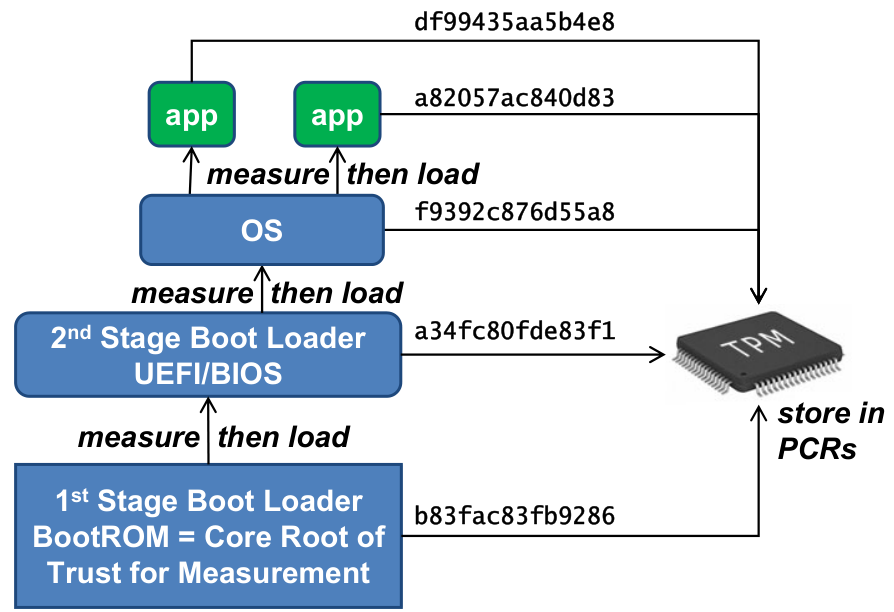
\includegraphics[width=0.4\textwidth]{img/measured-boot.png}
    \caption{Measured Boot}
\end{figure}

\subsection{Remote attestation procedure}

\begin{enumerate}
    \item challenge (=nonce)
    \item measurements (and nonce) signed with the device's key
    \item validate signature (crypto + ID) and check measurements against Reference Measurements (golden values)
\end{enumerate}

\subsection{Management of Remote Attestation}

Management of Remote Attestation involves several considerations. One of the first questions is whether to focus on \textbf{boot attestation} (static) or also include periodic (dynamic) attestation. It is essential to consider the attack model, particularly regarding runtime vulnerabilities, as well as the periodicity of the operation. The speed of an attack must also be taken into account, especially given the implementation limits, which include factors such as signature verification, protocol handling, and database lookups. Currently, the response time for these operations is in the range of several seconds, largely due to the inherent slowness of the TPM.

Another critical aspect is \textbf{whitelist generation}. This task can be challenging in general but becomes more manageable within limited environments, such as IoT, edge devices, Software-Defined Networking (SDN), and Network Function Virtualization (NFV). Labels for attestation states, such as "good," "old," "buggy," and "vulnerable," play a significant role in this process. Moreover, it is crucial to include configurations, which may come from management and orchestration frameworks (like MANO) or network management systems. Whitelist generation is typically easier when dealing with file-based configurations, but it becomes significantly more difficult when configurations are stored in memory.

\subsection{TCG PC Client PCR use}

\begin{figure}{ht}
    \centering
    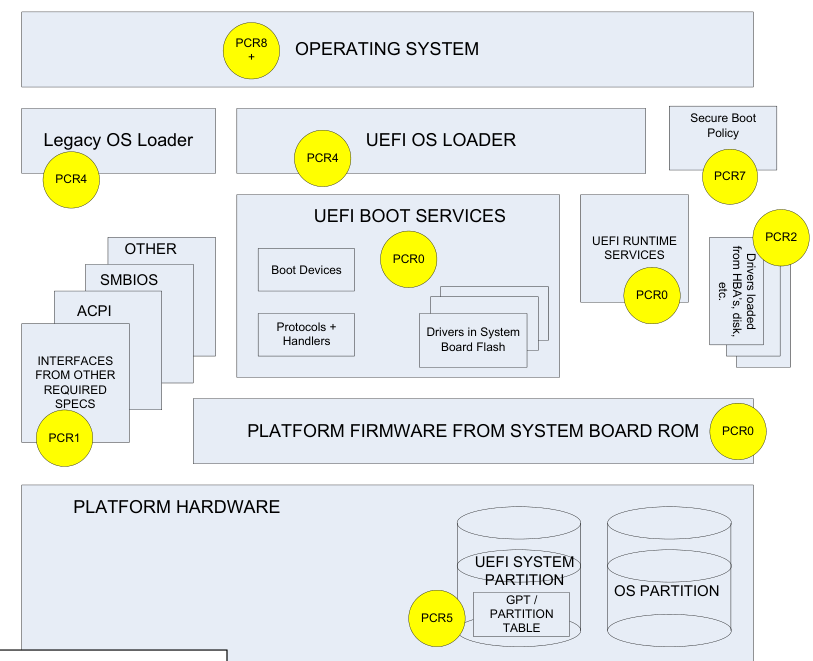
\includegraphics[width=0.4\textwidth]{img/tcg-pcr-arch.png}
    \caption{architecture of TCG PC Client}
\end{figure}

\begin{table}[h]
    \centering
    \caption{PCR Index and Usage}
    \begin{tabular}{lp{0.7\textwidth}}
        \toprule
        \textbf{PCR Index} & \textbf{PCR Usage} \\ \midrule
        0  & SRTM, BIOS, Host Platform Extensions, \newline Embedded Option ROMs and PI Drivers \\ 
        1  & Host Platform Configuration \\ 
        2  & UEFI driver and application Code \\ 
        3  & UEFI driver and application Configuration and Data \\ 
        4  & UEFI Boot Manager Code (usually the MBR) and Boot Attempts \\ 
        5  & Boot Manager Code Configuration and Data \newline (for use by the Boot Manager Code) and GPT/Partition Table \\ 
        6  & Host Platform Manufacturer Specific \\ 
        7  & Secure Boot Policy \\ 
        8-15 & Defined for use by the Static OS \\ 
        16 & Debug \\ 
        23 & Application Support \\ 
        \bottomrule
    \end{tabular}
\end{table}

\subsection{Measured execution}

In the context of measured execution, a notable \textbf{problem} arises: there are often not enough Platform Configuration Registers (PCRs) available to capture the necessary integrity measurements. A \textbf{solution} is to utilize just one PCR. However, this approach introduces a significant caveat: the PCR value now becomes dependent on the execution order of the measurements.


\subsection{Linux's IMA }
Linux’s Integrity Measurement Architecture (IMA) extends attestation capabilities to dynamic execution, such as applications. The process can be broken down into several key functions:
\begin{itemize}[itemsep=0pt]
\item \textbf{Collect}: IMA measures a file before it is accessed, ensuring that any changes to the file's integrity are detected early in the execution process.

\item \textbf{Store}: The measurement is then added to a kernel-resident list known as the Measurement List (ML) and is used to extend the IMA Platform Configuration Register (PCR), specifically PCR 10.

\item  \textbf{Appraise}: IMA can enforce local validation of a measurement against a “good” value, which is stored in an extended attribute of the file. This step ensures that only trusted files are executed in the system.

\item \textbf{Protect}: Finally, IMA protects a file's security extended attributes, including the appraisal hash, against offline attacks, thereby maintaining the integrity of the file's security features.
\end{itemize}

\subsubsection{Details}

Linux's Integrity Measurement Architecture (IMA) extends the concept of UEFI measured boot to the operating system and applications. It specifically uses PCR 10 for integrity measurements. The first measurement recorded is \textbf{boot\_aggregate}, which is a hash of the TPM’s PCRs 0 to 7 (i.e., UEFI-related PCRs). 

Measurement configuration is facilitated through the IMA template, primarily using the \textbf{ima-ng} format, though it can be customized to meet specific needs. These configurations are exposed in the kernel’s \texttt{securityfs} at the path \texttt{/sys/kernel/security/ima/ascii\_runtime\_measurements}.

\begin{table}[h]
    \centering
    \caption{IMA Measurement Records}
    \bigskip
    \begin{tabular}{@{}lllll@{}}
        \toprule
        \textbf{PCR} & \textbf{template\_hash} & \textbf{fitemplate} & \textbf{filedata-hash} & \textbf{filename-hint} \\ 
        \midrule
        10 & 91f34b5\ldots ab1e127  & ima-ng   & sha1:1801e1b\ldots 4eaf6b3 & boot\_aggregate\\ 
        10 & 8b16832\ldots e86486a & ima-ng  & sha256:efdd249\ldots b689954 & /init\\ 
        10 & ed893b1\ldots e71e4af & ima-ng &  sha256:1fd312a\ldots 6a6a524 & /usr/lib64/ld-2.16.so\\ 
        10 &  9051e8e\ldots 4ca432b & ima-ng & sha256:3d35533\ldots efd84b8 & /etc/ld.so.cache\\ 
        \bottomrule
    \end{tabular}
\end{table}

\subsection{Verification of the IMA ML}


With IMA enabled, the attestation report includes not only the nonce and PCR values but also the Measurement List (ML). However, the value of PCR 10 is variable; it depends on two factors: (A) the applications executed and (B) the order of execution of those applications. Consequently, the verifier must compute the correct value of PCR 10 by utilizing the ML.

The process can be outlined as follows:
\begin{itemize}
    \item myPCR10 = 0
    \item myPCR10 = Extend (boot\_aggregate)
    \item For each measure M of component C:
    \begin{itemize}
        \item If (C not authorized) then  alarm
        \item If (M different from gold\_measure(C)), then raise alarm
        \item myPCR10 = extend ( M )
    \end{itemize}
    \item If myPCR10 equals PCR10, then OK, else alarm
\end{itemize}

In summary, this verification process ensures that the components executed on the system are authorized and that their measurements match the expected values, thereby maintaining the integrity of the system.


\subsection{Size and variability of the TCB}

The Trusted Computing Base (TCB) represents the smallest amount of code, hardware, personnel, and processes that must be trusted to fulfill security requirements. Confidence in the TCB can be enhanced through various means, including static verification, code inspection, testing, and formal methods. However, all these methods tend to be expensive, making it crucial to reduce the complexity of the TCB. Nevertheless, simply reducing complexity is not sufficient on its own.

The Trusted Platform Module (TPM) attempts to establish a TCB via the Core Root of Trust for Measurement (CRTM). Despite these efforts, the TCB has often become too large and excessively dynamic. Consequently, two “identical” computers may yield different measurements, which complicates the assurance of trustworthiness across systems.

\subsection{Dynamic Root of Trust for Measurement}

The Dynamic Root of Trust for Measurement (DRTM) offers an alternative approach by not trusting all operations that occur since the BIOS. Instead, it resets the CPU and begins measuring from that point onward. In this context, TPM version 1.2 introduced dynamic Platform Configuration Registers (PCRs), specifically PCRs 17 to 23, which are initially set to -1 upon boot. These dynamic PCRs can subsequently be reset by the operating system to 0 when necessary.

DRTM utilizes special processor commands, such as \texttt{SENTER} for Intel TXT, which executes the SINIT binary module, and \texttt{SKINIT} for AMD SVM. This mechanism halts all processing on the platform, allowing DRTM to hash the contents of a designated memory region and store the measurement in the dynamic PCR. Control is then transferred to a specified location in memory. This process is also referred to as Late Launch.

One of the significant advantages of DRTM is its ability to address the problem of incorrect PCR values when firmware is updated, which can lead to issues with sealed data. By establishing a new root of trust at a later stage, DRTM helps ensure the integrity of the platform even amidst changes to the firmware.

\subsection{Hypervisor TEE}

The Dynamic Root of Trust for Measurement (DRTM) was designed to facilitate the loading of a hypervisor, such as Xen or VMware ESX. Once the hypervisor is loaded, it can isolate virtual machines (VMs) effectively. The Trusted Platform Module (TPM) plays a crucial role in attesting the hypervisor, ensuring that it has been loaded properly before allowing access to TPM sealed storage. This capability may prove particularly beneficial in cloud computing environments, where security and isolation are paramount. However, it is important to note that the hypervisor itself comprises a substantial amount of code that must be validated. For instance, Xen includes a complete copy of Linux, while VMware is of a similar scale, which raises concerns regarding the potential attack surface.

\subsection{RA in Virtualized Environments}

Having a hardware Root of Trust (RoT) is a critical aspect of security in virtualized environments. In the case of full virtualization, such as with virtual machines (VMs), there is often only a software implementation of the RoT, exemplified by virtual Trusted Platform Modules (vTPMs) provided by platforms like Xen, Google, and VMware. To enhance security, it is essential to establish a strong link between the vTPM and the physical TPM (pTPM).

One promising approach to achieve this is through deep attestation, which leverages hardware-based security. This method involves using sealed objects that are rooted in the pTPM to protect the vTPM. However, implementing this strategy requires an extension of the standard interfaces defined by the Trusted Computing Group (TCG), and this is currently an ongoing area of development.

In contrast, when adopting lighter forms of virtualization, such as Docker containers, a different solution becomes feasible. Since hardware, including the TPM, is shared among containers, this allows for alternative security mechanisms that can still ensure the integrity and confidentiality of applications without the overhead associated with full virtualization.

\subsection{RA for OCI Containers}

Remote Attestation (RA) for Open Container Initiative (OCI) containers is designed to be agnostic, meaning it is not tied to a specific containerization technology. This approach ensures that RA is transparent to both the container runtime and the containerized workloads, allowing for seamless integration. The RA process provides assurance of the integrity of the host system along with the containers themselves, leveraging a hardware Root of Trust (RoT) to establish a secure and trusted environment.

\begin{figure}{ht}
    \centering
    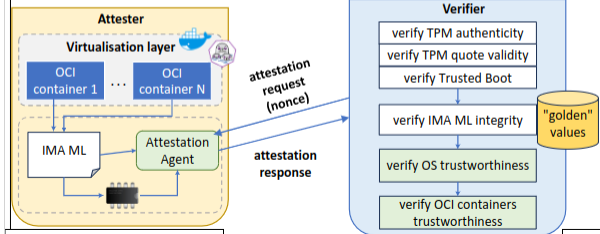
\includegraphics[width=0.4\textwidth]{img/ra-oci.png}
    \caption{RA for OCI Containers}
\end{figure}


\subsubsection{Implementation}

The implementation of Remote Attestation (RA) for Open Container Initiative (OCI) containers involves the introduction of a new Integrity Measurement Architecture (IMA) template known as \texttt{ima-dep-cgn}. This template is designed to assess the dependencies of entries, determining whether they belong to the host or to a specific container. 

A key feature of this implementation is the inclusion of a \texttt{control-group-name}, which uniquely identifies the container in question. Furthermore, the \texttt{template-hash} is computed using a digest algorithm other than SHA-1, allowing for the use of more secure hashing methods such as SHA-256 or SHA-512. This enhances the overall integrity and security of the RA process for OCI containers.
